\documentclass{beamer}
\usetheme{Berkeley}
\usecolortheme{dolphin}

\usepackage[utf8]{inputenc}
\usepackage{amsmath, amssymb, hyperref, multirow, dot2texi}

\usepackage{tikz}
\usetikzlibrary{shapes, arrows}

\title{Using scores to improve language modelling of movie plot summaries}
\author[J. Sáez Gómez, R. vd Heijden, F. Stablum]{Jorge Sáez Gómez\\Roelof van der Heijden\\Francesco Stablum}
\institute{Universiteit van Amsterdam}
\date{\today}

\begin{document}

\begin{frame}
	\maketitle
\end{frame}

\begin{frame}{Presentation outline}
	\tableofcontents
\end{frame}

\section{Problem formulation}

\begin{frame}{Problem formulation}
	\begin{itemize}
	\item Is there any correlation between the score of a movie and the contents of its script?
	\item Can we use the score to better model a movie corpus?
	\end{itemize}
\end{frame}

\section{Models}

\begin{frame}{Models}
	Latent Dirichlet Allocation:\footnote{\tiny{}Image taken from the paper ``Supervised topic models'' by David M. Blei and Jon D. McAuliffe (2007)}

	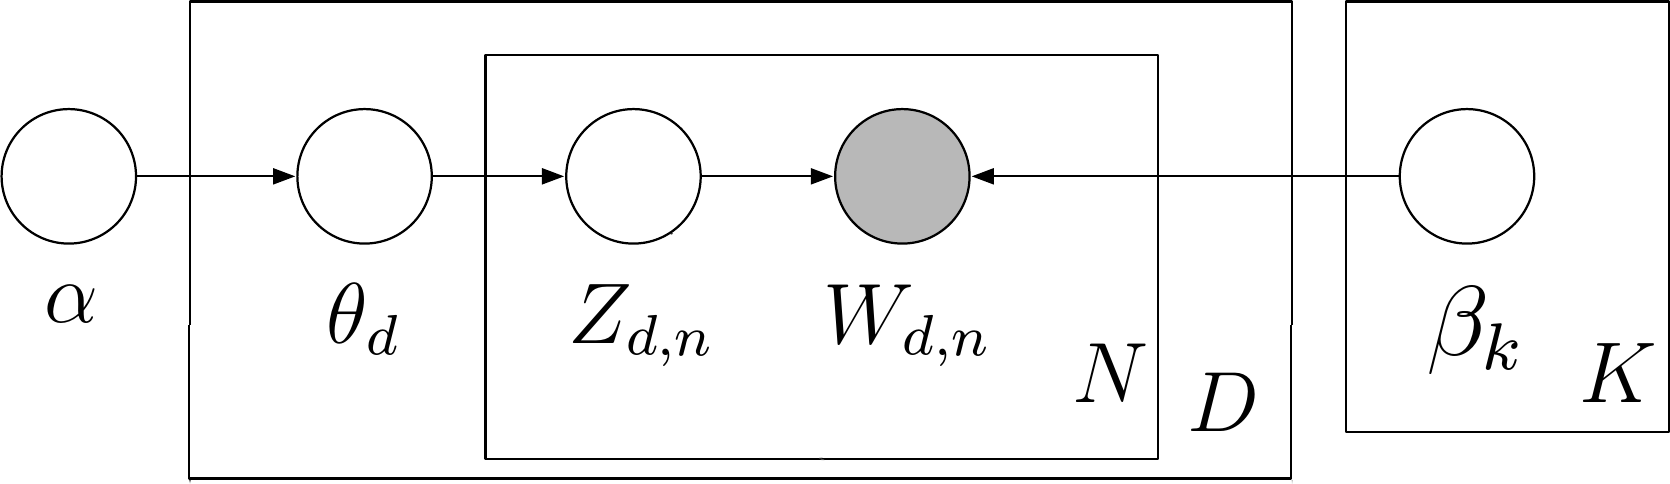
\includegraphics[width=\textwidth]{LDA.png}
\end{frame}

\begin{frame}{Models}
	Supervised Latent Dirichlet Allocation:\footnote{\tiny{}Image taken from the paper ``Supervised topic models'' by David M. Blei and Jon D. McAuliffe (2007)}

	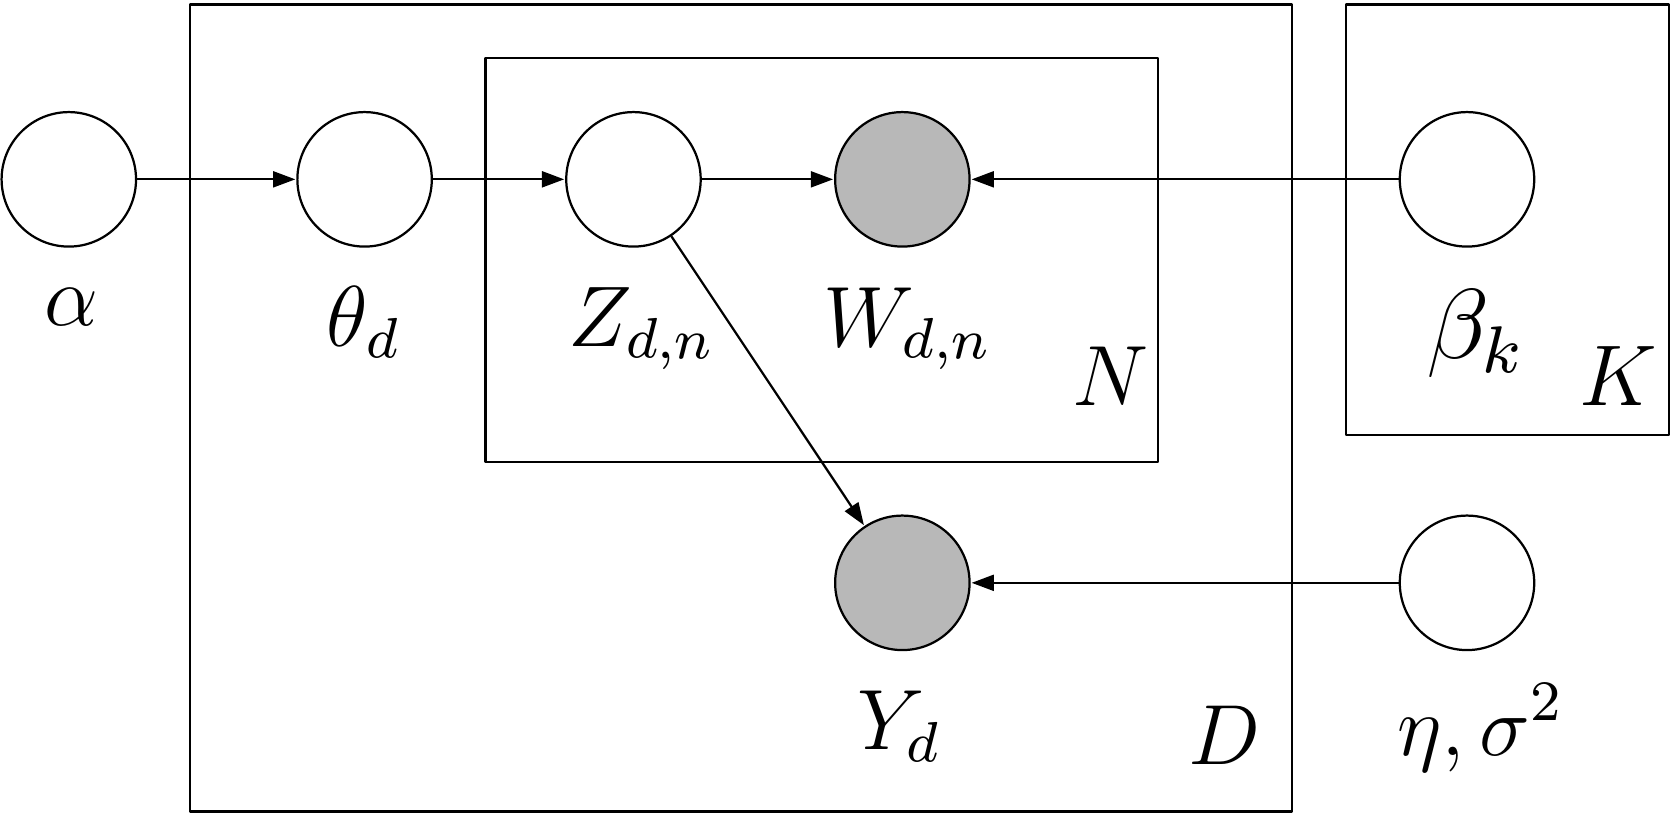
\includegraphics[width=\textwidth]{SLDA.png}
\end{frame}

\section{Approach}

\begin{frame}{Approach}
	Our collapsed Gibbs sampler:
	\begin{multline*}
	p(z_{di} = k \mid Z^{\backslash i}, S, W, \alpha, \beta, \eta, \sigma) \propto \\
	\left[ \prod_{k'} \frac{\prod_w \Gamma(N_{{k'}w}^{\backslash i} + \mathbb{I}(k' = k \wedge w = w_{di}) + \beta)}{\Gamma(N_{k'}^{\backslash i} + \mathbb{I}(k' = k) + W \beta)} \right] \times \\
	\underbrace{\mathcal{N}\left(s_d\, \left|\, \eta^T \cdot \frac{N_{d{k'}}^{\backslash i} + \mathbb{I}(k' = k)}{N_d}, \sigma\right. \right)}_\text{Movie score term} \prod_{k'} \Gamma(N_{d{k'}}^{\backslash i} + \mathbb{I}(k' = k) + \alpha)
	\end{multline*}
	Better implemented in log-space probabilities to avoid numerical problems.
\end{frame}

\begin{frame}{Approach}
	Estimating the global score hyperparameter $\eta$:
	\begin{multline*}
	\eta_k^{new} \leftarrow (1 - \gamma) \eta_k^{old} + \gamma \frac{\sum_d \frac{N_{dk}}{N_d} \left( s_d - \sum_{k' \ne k} \eta_{k'}^{old} \frac{N_{dk'}}{N_d} \right)}{\sum_d \left( \frac{N_{dk}}{N_d}  \right)^2 + \varepsilon}
	\end{multline*}
	
	Where:
	\begin{itemize}
	\item $1 \gg \gamma > 0$ in order for the previous series to converge.
	\item $1 \gg \varepsilon > 0$ is a smoothing constant.
	\end{itemize}
\end{frame}

\section{Dataset}

\begin{frame}{Dataset}
	\begin{itemize}
	\item We made scripts to crawl \url{http://www.imsdb.com/} for movie scripts and then search \url{http://www.imdb.com/} for movie scores and plot summaries.
	\item We got a database with $\approx$ 700 movies.
	\item Movie score distribution (from 0 to 10):
	\end{itemize}

	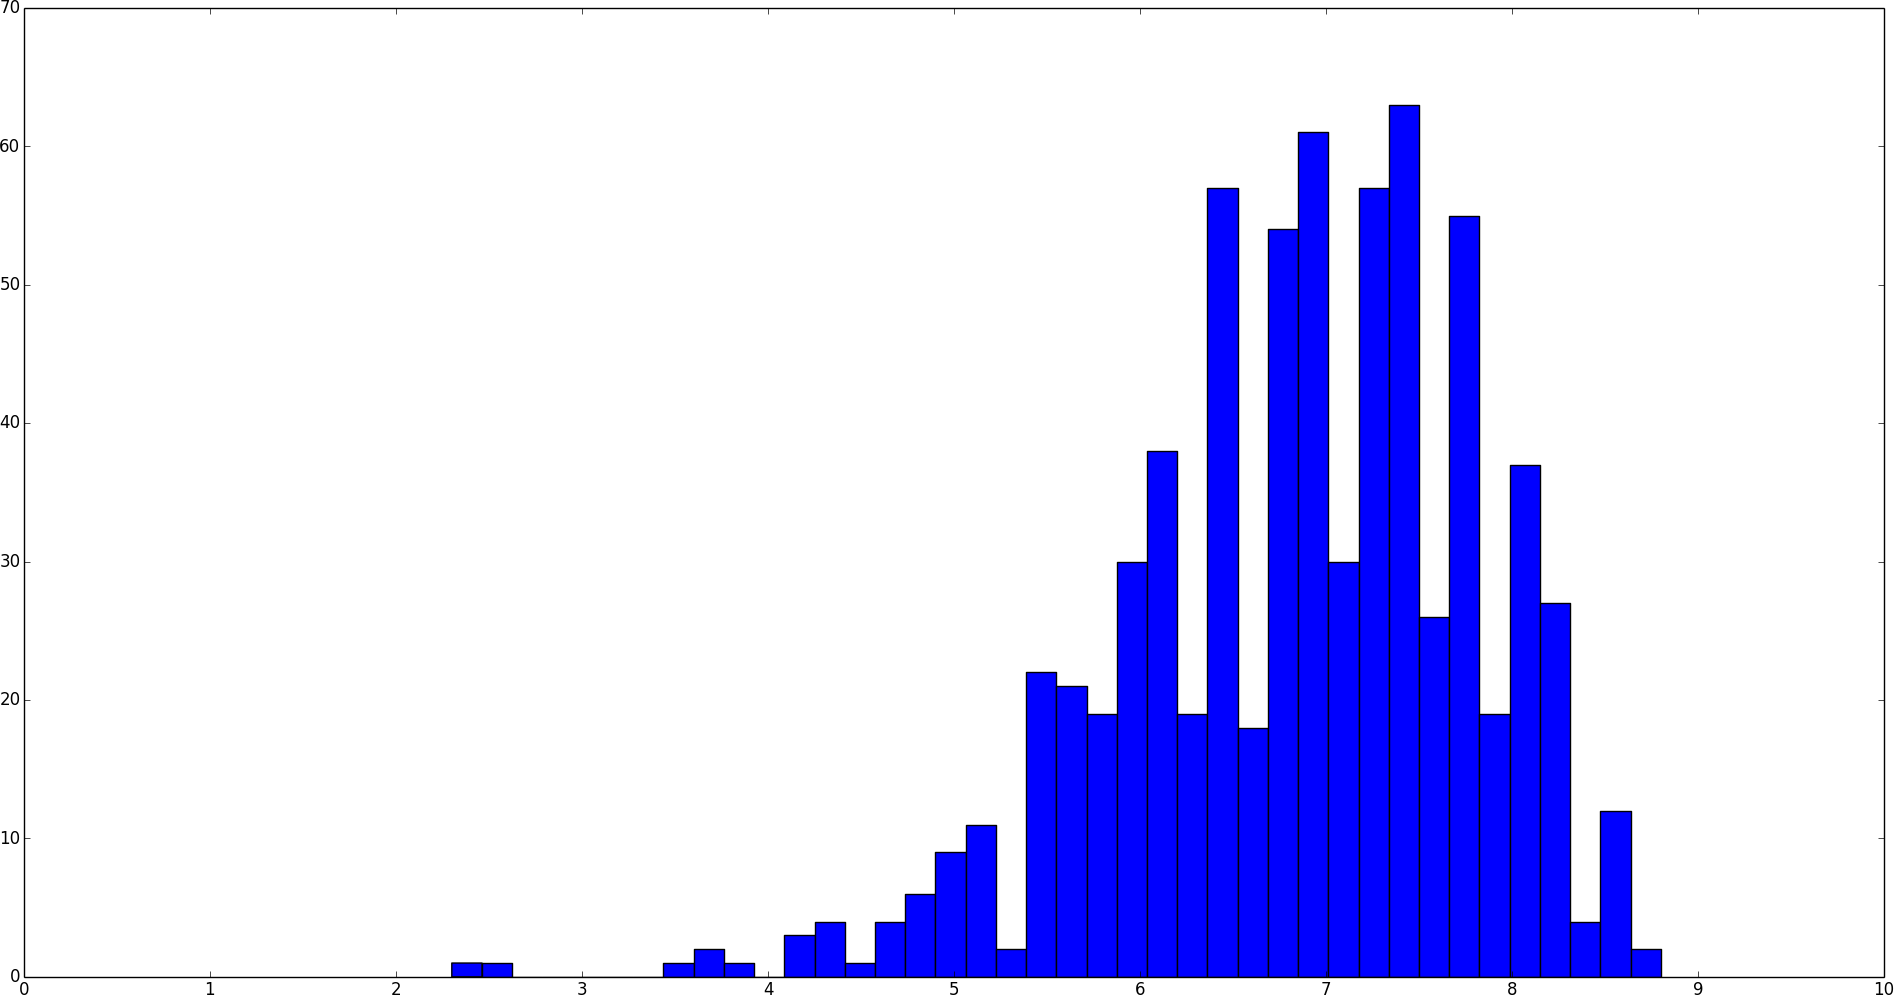
\includegraphics[width=\textwidth]{scores_histogram.png}
\end{frame}

\begin{frame}{Dataset}
	\begin{itemize}
	\item Tokenization $\rightarrow$ stemming $\rightarrow$ pruning
	\item We prune words appearing only on a single movie (avoids overfitting) or within a stop list.
	\item Total number of tokens $\approx 12.7 \cdot 10^6$
	\item Number of unique tokens $\approx$ 35000
	\item Average number of tokens within a movie summary $\approx$ 75
	\item Average number of tokens within a movie script $\approx$ 18000
	\end{itemize}
\end{frame}

\section{Results}

\begin{frame}{Results}
	\begin{itemize}
	\item Initial selection of 120 movies (100 training / 20 testing) with balanced scores.
	\item Perplexity measure:
	
	\begin{center}
	\begin{tabular}{cc|ccc}
		LDA topics      & & 25 & 50 & 100 \\ \hline
		\multirow{2}{*}{Using scores?} & No  & 4128 & 5333 & 6954 \\
		                               & Yes & \textbf{4005} & 5503 & 7082 \\
	\end{tabular}
	\end{center}
	
	\item Inverse accuracy measure:
	
	\begin{center}
	\begin{tabular}{cc|ccc}
		LDA topics      & & 25 & 50 & 100 \\ \hline
		\multirow{2}{*}{Using scores?} & No  & 845 & 1318 & 2049 \\
		                               & Yes & \textbf{805} & 1372 & 2067 \\
	\end{tabular}
	\end{center}
	\end{itemize}
\end{frame}

\section{Discussion}

\begin{frame}{Discussion}
	\begin{itemize}
	\item Use of few movies $\Rightarrow$ the model starts overfitting with 50-100 topics already.
	\item Slight predictive improvement if using movie scores, but it is not significant.
	\end{itemize}
\end{frame}

\section{Challenges}

\begin{frame}{Challenges}
	\begin{itemize}
	\item Improve speed of the collapsed Gibbs sampler.
	\item Use the movie scripts instead of the movie summaries.
	\item Use both the movie scripts and summaries.
	\item Incorporate more information into the model, such as the movie genre.
	\end{itemize}
\end{frame}

\end{document}
